\documentclass[11pt,a4paper]{article}

\usepackage[utf8]{inputenc}
\usepackage[T1]{fontenc}
\usepackage{lmodern}
\usepackage[english]{babel}
\usepackage[margin=2.5cm]{geometry}
\usepackage{amsmath}
\usepackage{graphicx}
\usepackage{xcolor}
\usepackage{listings}
\usepackage{booktabs}
\usepackage{enumitem}
\usepackage{caption}
\usepackage{float}
\usepackage{tikz}
\usetikzlibrary{arrows.meta,positioning,shapes.geometric,calc,fit}
\usepackage[hidelinks]{hyperref}

\captionsetup{font=small,labelfont=bf}
\setlength{\parskip}{0.5em}
\setlength{\parindent}{0pt}

\lstset{
  basicstyle=\ttfamily\footnotesize,
  breaklines=true,
  breakatwhitespace=false,
  frame=single,
  rulecolor=\color{black!30},
  backgroundcolor=\color{black!3},
  columns=fullflexible,
  keepspaces=true,
  showstringspaces=false,
  commentstyle=\color{green!40!black},
  numbers=none,
  xleftmargin=0pt,
  aboveskip=0.8em,
  belowskip=0.4em
}
\lstdefinestyle{py}{language=Python,keywordstyle=\color{blue!60!black}\bfseries,commentstyle=\color{green!40!black}\itshape}
\lstdefinestyle{sh}{language=bash}

\newcommand{\code}[1]{\texttt{#1}}
\newcommand{\hh}[1]{$h_{#1}$}

\begin{document}

%--------------------------------------------------------------------
% Title page
%--------------------------------------------------------------------
\begin{titlepage}
\centering
\vspace*{0.5cm}

\includegraphics[width=0.85\linewidth]{figures/logos.png}\\[1.5cm]
{\Large Department of Information Engineering, Computer Science\\and Mathematics (DISIM)}\\[2cm]
{\huge\bfseries SDN Project:\\[0.3em] Ring Topology and Filtering Policies\\[0.3em] in a Kathar\'a Environment}\\[2cm]
{\large Supervisor: Prof.\ Carlo Centofanti}\\[0.8cm]
{\large Student: Diego Banfi}\\[0.8cm]
{\large Academic Year 2025--2026}\\[2cm]
{\small Source code: \url{https://github.com/Diegobanfi/progetto-sdn-kathara}}
\vfill
\end{titlepage}

\tableofcontents
\clearpage

%====================================================================
\section{Introduction and Topology Changes}
%====================================================================
The goal of this project is to extend and improve an existing
Software-Defined Networking (SDN) network. The starting infrastructure
implemented a traditional Layer-2 learning-switch behaviour, centrally
controlled through the Ryu framework. It has been modified both in its
topology and in its control logic.

The work is organised in three tasks:
\begin{enumerate}
  \item \textbf{Topology extension:} add a third SDN switch ($s_3$) to close a
        redundant ring between the core switches.
  \item \textbf{Firewall:} implement a proactive traffic-filtering policy that
        isolates an unauthorised host directly in the data plane.
  \item \textbf{Policy routing:} steer one unicast flow over an alternative path
        that uses the new link, bypassing the default path.
\end{enumerate}

%====================================================================
\section{Task 1: Creating the SDN Ring}
%====================================================================
In the original topology the Open vSwitch (OVS) switches forwarded traffic over
a linear connection. To introduce fault tolerance and the ability to balance
load, the OpenFlow switch $s_3$ was added. It is directly connected to both
$s_1$ (core) and $s_2$ (access), which creates a ring (a physical loop) inside
the SDN domain.

In a local network made of legacy switches such a topology would immediately
cause a broadcast storm, saturating the links and bringing the infrastructure
down unless the Spanning Tree Protocol (STP) were running. In the SDN paradigm
the loop is instead handled deterministically in software, through control of
the flow tables.

\begin{figure}[H]
\centering
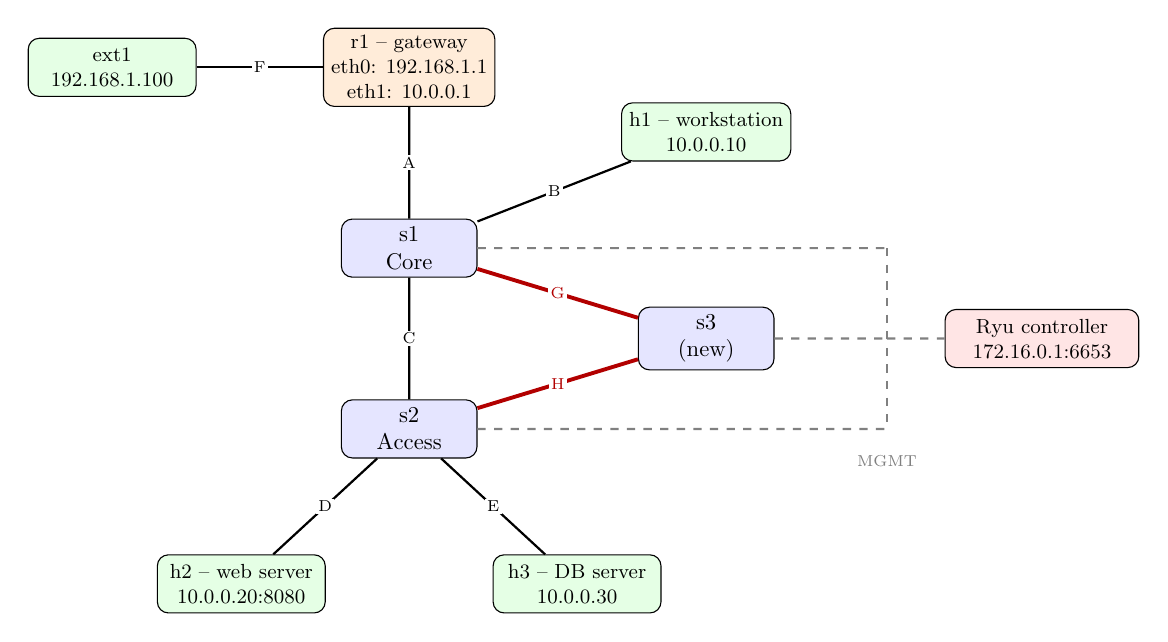
\begin{tikzpicture}[scale=0.82, every node/.style={transform shape},
  sw/.style={draw,rounded corners,fill=blue!10,minimum width=2.1cm,minimum height=0.9cm,align=center},
  host/.style={draw,rounded corners,fill=green!10,minimum width=2.6cm,minimum height=0.9cm,align=center,font=\small},
  rt/.style={draw,rounded corners,fill=orange!15,minimum width=2.6cm,minimum height=0.9cm,align=center,font=\small},
  ctl/.style={draw,rounded corners,fill=red!10,minimum width=3.0cm,minimum height=0.9cm,align=center,font=\small},
  lbl/.style={font=\scriptsize,fill=white,inner sep=1pt},
  link/.style={thick},
  mgmt/.style={thick,dashed,gray}
]
\node[host] (ext) at (0,0) {ext1\\192.168.1.100};
\node[rt]   (r1)  at (4.6,0) {r1 -- gateway\\eth0: 192.168.1.1\\eth1: 10.0.0.1};
\node[sw]   (s1)  at (4.6,-2.8) {s1\\Core};
\node[host] (h1)  at (9.2,-1.0) {h1 -- workstation\\10.0.0.10};
\node[sw]   (s3)  at (9.2,-4.2) {s3\\(new)};
\node[sw]   (s2)  at (4.6,-5.6) {s2\\Access};
\node[host] (h2)  at (2.0,-8.0) {h2 -- web server\\10.0.0.20:8080};
\node[host] (h3)  at (7.2,-8.0) {h3 -- DB server\\10.0.0.30};
\node[ctl]  (ct)  at (14.4,-4.2) {Ryu controller\\172.16.0.1:6653};

\draw[link] (ext) -- node[lbl]{F} (r1);
\draw[link] (r1)  -- node[lbl]{A} (s1);
\draw[link] (s1)  -- node[lbl]{B} (h1);
\draw[link] (s1)  -- node[lbl]{C} (s2);
\draw[link,red!70!black,line width=1.4pt] (s1) -- node[lbl]{G} (s3);
\draw[link,red!70!black,line width=1.4pt] (s2) -- node[lbl]{H} (s3);
\draw[link] (s2)  -- node[lbl]{D} (h2);
\draw[link] (s2)  -- node[lbl]{E} (h3);

% management bus
\draw[mgmt] (12.0,-2.8) -- (12.0,-5.6);
\draw[mgmt] (s1.east |- 12.0,-2.8) -- (12.0,-2.8);
\draw[mgmt] (s1.east) -- (12.0,-2.8);
\draw[mgmt] (s2.east) -- (12.0,-5.6);
\draw[mgmt] (s3.east) -- (12.0,-4.2);
\draw[mgmt] (12.0,-4.2) -- (ct.west);
\node[lbl,text=gray] at (12.0,-6.1) {MGMT};
\end{tikzpicture}
\caption{Extended SDN topology with a ring between $s_1$, $s_2$ and $s_3$.
Solid lines are the data plane, dashed lines the out-of-band management plane
towards the Ryu controller (the controller is attached to the shared MGMT
domain, which also reaches $s_1$, $s_2$, $s_3$). Domains \textbf{G} and
\textbf{H} (red) are the new collision domains introduced to close the ring.}
\label{fig:topology}
\end{figure}

The only new interfaces with respect to the starting topology are those needed
to attach $s_3$ to the rest of the network:
\begin{itemize}
  \item Domain G: \code{s1:eth4} $\leftrightarrow$ \code{s3:eth0}
  \item Domain H: \code{s2:eth4} $\leftrightarrow$ \code{s3:eth1}
  \item Management: \code{controller} $\leftrightarrow$ \code{s3:eth2}
\end{itemize}

\subsection{Changes to \texttt{lab.conf} and the \texttt{.startup} files}
To integrate $s_3$ and close the logical ring, changes were made both to the
global configuration file \code{lab.conf} and to the \code{.startup} files of
$s_1$ and $s_2$. Only the lines added with respect to the linear starting
topology (without the third switch) are shown below.

\subsubsection{Changes to \texttt{lab.conf}}
In the original configuration $s_1$ and $s_2$ were connected only through
collision domain C. The following lines were added:

\begin{lstlisting}[style=sh,caption={Lines added to \texttt{lab.conf} to insert $s_3$}]
# --- Core SDN Switch (s1) ---
s1[4]="G"      # NEW: interface eth4, towards s3

# --- Access SDN Switch (s2) ---
s2[4]="H"      # NEW: interface eth4, towards s3

# --- New SDN Switch (s3) ---
s3[image]="kathara/sdn"
s3[0]="G"      # towards s1 (eth0)
s3[1]="H"      # towards s2 (eth1)
s3[2]="MGMT"   # management interface (eth2)
\end{lstlisting}

The lines \code{s1[4]="G"} and \code{s2[4]="H"} give $s_1$ and $s_2$ a new
Ethernet interface (\code{eth4}) attached to the two new collision domains G and
H. The \code{s3[...]} block fully defines the new node, with two data interfaces
(\code{eth0}, \code{eth1}) towards the ring and one management interface
(\code{eth2}).

\subsubsection{Changes to \texttt{s1.startup} and \texttt{s2.startup}}
In the startup file of $s_1$ the new \code{eth4} interface was added to the
Open vSwitch bridge, corresponding to the new OpenFlow port towards $s_3$:

\begin{lstlisting}[style=sh,caption={Line added to \texttt{s1.startup}}]
ovs-vsctl add-port s1 eth4   # NEW: OF port 4, towards s3
\end{lstlisting}

Likewise, \code{s2.startup} received the \code{eth4} interface towards $s_3$:

\begin{lstlisting}[style=sh,caption={Line added to \texttt{s2.startup}}]
ovs-vsctl add-port s2 eth4   # NEW: OF port 4, towards s3
\end{lstlisting}

\subsubsection{New file \texttt{s3.startup}}
Since $s_3$ is a completely new node, its startup file was written from scratch.
It follows the same scheme as the other two switches: start the Open vSwitch
service, create the bridge, add the two data ports, configure the management
interface and connect to the Ryu controller.

\begin{lstlisting}[style=sh,caption={Contents of \texttt{s3.startup}}]
# s3.startup - new SDN switch (ring)
# Data ports: eth0 -> s1, eth1 -> s2
# Management: eth2 -> controller (NOT added to the OVS bridge)

/etc/init.d/openvswitch-switch start

ovs-vsctl add-br s3

ovs-vsctl add-port s3 eth0
ovs-vsctl add-port s3 eth1

ip link set eth0 up
ip link set eth1 up

ip addr add 172.16.0.30/24 dev eth2
ip link set eth2 up

ovs-vsctl set bridge s3 other-config:datapath-id=0000000000000003

ovs-vsctl set-controller s3 tcp:172.16.0.1:6653
\end{lstlisting}

\begin{itemize}
  \item \textbf{Bridge creation and data plane:} \code{add-br s3} creates the
        logical bridge that represents the Open vSwitch switch. The two
        \code{add-port} commands attach the data interfaces: \code{eth0} is
        connected to $s_1$ through domain G, \code{eth1} to $s_2$ through
        domain H. From this point both interfaces are handled by Open vSwitch as
        data-plane ports.
  \item \textbf{Out-of-band management channel:} \code{eth2}, attached to the
        isolated MGMT domain, receives the static address
        \code{172.16.0.30/24}. It is \emph{not} added to the bridge, so it does
        not take part in data-plane forwarding and is used only to talk to the
        Ryu controller.
  \item \textbf{Control-plane connection:} \code{ovs-vsctl set-controller s3
        tcp:172.16.0.1:6653} makes Ryu the OpenFlow controller of the switch
        (address \code{172.16.0.1}, TCP port \code{6653}). After this, $s_3$
        receives from the controller the forwarding rules needed for routing and
        SDN policies.
  \item \textbf{Datapath ID:} \code{other-config:datapath-id} assigns the DPID
        \code{0000000000000003} to $s_3$, which lets Ryu tell it apart from the
        other switches and apply the right OpenFlow rules to each device.
\end{itemize}

\subsubsection{Note: Kathar\'a indices, Linux interfaces and OpenFlow ports}
Three different numberings must be kept apart: the Kathar\'a index, the Linux
interface name and the OpenFlow port. The line in \code{lab.conf}
\begin{lstlisting}[style=sh]
s1[4]="G"
\end{lstlisting}
creates the Linux interface \code{eth4} on node $s_1$ and attaches it to
collision domain G, which connects $s_1$ to $s_3$:
\[
  \code{s1:eth4} \leftrightarrow \text{G} \leftrightarrow \code{s3:eth0}
\]
For the SDN controller to use this interface it is added to the Open vSwitch
bridge:
\begin{lstlisting}[style=sh]
ovs-vsctl add-port s1 eth4
\end{lstlisting}
In the lab, the data ports of $s_1$ are added in the order \code{eth0},
\code{eth1}, \code{eth2}, \code{eth4}. OVS therefore assigns OpenFlow port~4 to
\code{eth4}.

\begin{table}[H]
\centering
\begin{tabular}{llc}
\toprule
Interface & Connected to & OpenFlow port\\
\midrule
\code{eth0} & r1 & 1\\
\code{eth1} & h1 & 2\\
\code{eth2} & s2 & 3\\
\code{eth4} & s3 & 4\\
\bottomrule
\end{tabular}
\caption{Data ports of $s_1$}
\end{table}

The number in the name \code{eth4} does \emph{not} determine the OpenFlow port
number: the name comes from Kathar\'a, whereas the OpenFlow port is assigned by
OVS when the interface is added to the bridge. \code{eth3} does not appear in
the table because it is used only for the management network and is not added to
the OVS bridge, so it never forwards data-plane packets. The mapping can be
checked with:
\begin{lstlisting}[style=sh]
ovs-vsctl get Interface eth4 ofport
\end{lstlisting}
which returns OpenFlow port 4 here.

%====================================================================
\section{Task 2: Selective Stateless Layer-3 Firewall}
%====================================================================
The second task implements a security policy in the data plane of the SDN
domain. The policy completely blocks IP communication between the workstation
$h_1$ (10.0.0.10) and the database server $h_3$ (10.0.0.30), while keeping the
web server $h_2$ (10.0.0.20) reachable from both endpoints and from the outside.

\subsection{Layer-3 filtering in SDN}
The main advantage of the SDN architecture is the separation between the control
plane and the data plane. The Ryu controller is the central point where network
policies are defined, while the Open vSwitch switches enforce them on packets.

For the firewall, the controller decides that traffic between $h_1$ and $h_3$
must be blocked. This decision is taken centrally and then translated into an
OpenFlow rule installed directly in the flow table of the relevant switch. Once
the rule is installed the controller no longer needs to inspect every packet:
the switch applies it autonomously. Subsequent packets are dropped in the data
plane without being sent to the controller again, which reduces the number of
messages on the control channel and the latency of later packets.

The policy works in three phases:
\begin{enumerate}
  \item \textbf{Reactive phase (first packet).} When $h_1$ sends its first IP
        packet towards $h_3$ (or vice versa), the switch has no specific rule
        for that traffic. The packet hits the table-miss rule, priority~0, and
        is sent to Ryu in an \code{OFPT\_PACKET\_IN} message.
  \item \textbf{Centralised decision.} The Ryu application parses the packet,
        reads the source and destination IPv4 addresses and checks whether the
        traffic belongs to the forbidden $h_1\leftrightarrow h_3$ communication.
        Since it must be blocked, the controller does not forward the packet and
        sends the switch an \code{OFPT\_FLOW\_MOD} installing a DROP rule with
        priority~300.
  \item \textbf{Autonomous phase (subsequent packets).} Once the rule is in
        place, the switch recognises later packets of the same flow by itself.
        The priority-300 rule is applied directly from the flow table and the
        packet is discarded without involving the controller, which reduces
        latency and control-channel traffic and leaves the controller free to
        handle other network events.
\end{enumerate}

\subsection{Firewall implementation in the controller}
For Task~2 only the Python file of the Ryu application was modified. The policy
blocks IPv4 traffic between $h_1$ and $h_3$ in both directions. The check is
performed in the method \code{\_packet\_in\_handler()}, i.e.\ the function Ryu
calls when a switch sends the controller a packet that does not match any rule
already present in its flow table.

\begin{lstlisting}[style=py,caption={Firewall block of Task 2}]
# IP addresses used by the policy
IP_H1 = "10.0.0.10"
IP_H3 = "10.0.0.30"

# Firewall H1 <-> H3
ip_pkt = pkt.get_protocol(ipv4.ipv4)
if ip_pkt:
    src_ip = ip_pkt.src
    dst_ip = ip_pkt.dst

    if ((src_ip == IP_H1 and dst_ip == IP_H3) or
            (src_ip == IP_H3 and dst_ip == IP_H1)):
        self.logger.warning("FIREWALL DROP: %s <-> %s", src_ip, dst_ip)

        match = parser.OFPMatch(
            eth_type=0x0800,
            ipv4_src=src_ip,
            ipv4_dst=dst_ip
        )

        self._add_flow(
            datapath,
            priority=300,
            match=match,
            actions=[]
        )
        return
\end{lstlisting}

The constants \code{IP\_H1} and \code{IP\_H3} identify the endpoints involved in
the security policy: the first holds the address of workstation $h_1$
(10.0.0.10), the second that of database server $h_3$ (10.0.0.30). The
statement
\begin{lstlisting}[style=py]
ip_pkt = pkt.get_protocol(ipv4.ipv4)
\end{lstlisting}
extracts the IPv4 header from the received packet. If the packet is not IPv4,
\code{ip\_pkt} is empty and the firewall block is skipped; this lets ARP traffic,
which is needed to resolve MAC addresses, be handled separately. The condition
\code{if ip\_pkt:} therefore checks that the packet really contains an IPv4
header before its fields are accessed, and the following two statements extract
the source and destination IP addresses.

The main firewall condition checks both directions of the communication: the
first part covers traffic from $h_1$ to $h_3$, the second traffic from $h_3$ to
$h_1$. The policy is therefore bidirectional: IP communication cannot be started
in either direction. The \code{logger.warning(...)} call writes a message to the
controller log, which is useful during testing to confirm that Ryu recognised
and blocked the forbidden traffic.

The \code{match} variable defines the fields the switch must compare.
\code{eth\_type=0x0800} selects Ethernet frames carrying IPv4, while
\code{ipv4\_src} and \code{ipv4\_dst} make the rule specific to the
source--destination pair that violated the policy.

The call to \code{\_add\_flow(...)} sends the switch an OpenFlow
\code{OFPT\_FLOW\_MOD} message that installs a new rule in its flow table.
\code{datapath} identifies the switch on which the rule is installed.
\code{priority=300} gives the firewall policy a higher priority than the
policy-routing rules (priority~200), the MAC-learning rules (priority~1) and the
table-miss rule (priority~0). \code{actions=[]} is the DROP action: OpenFlow has
no explicit DROP action; if a rule matches but contains no forwarding action,
the packet is discarded. Finally, \code{return} stops the execution of
\code{\_packet\_in\_handler()} for the current packet. The first packet is thus
blocked by the controller, while all following packets are blocked directly by
the flow rule installed in the switch.

%====================================================================
\section{Task 3: Policy Routing on the Ring}
%====================================================================
The goal of Task~3 is an \emph{asymmetric} policy routing in which the Ryu
controller no longer merely forwards packets according to MAC learning, but
deliberately decides which path they follow, based on source and destination IP
addresses:
\begin{itemize}
  \item \textbf{Forward path $h_1\to h_2$:} traffic follows
        $h_1\to s_1\to s_3\to s_2\to h_2$.
  \item \textbf{Return path $h_2\to h_1$:} traffic follows the direct path
        $h_2\to s_2\to s_1\to h_1$.
  \item The existing firewall policy between $h_1$ and $h_3$ must be kept.
\end{itemize}

\subsection{Logical architecture of the controller}
Task~3 integrates several components in the same Ryu application: the Task~2
firewall rules, IPv4 policy routing, handling of ARP requests on the ring, and a
fallback MAC-learning behaviour. Figure~\ref{fig:flowchart} shows the logical
order in which the controller examines a packet received through a
\code{PacketIn} message. The following sections describe each block in detail.
In short, the static flows handle IPv4 traffic between $h_1$ and $h_2$, while
the ARP logic controls how broadcasts propagate over the inter-switch links to
avoid Layer-2 loops.

\begin{figure}[H]
\centering
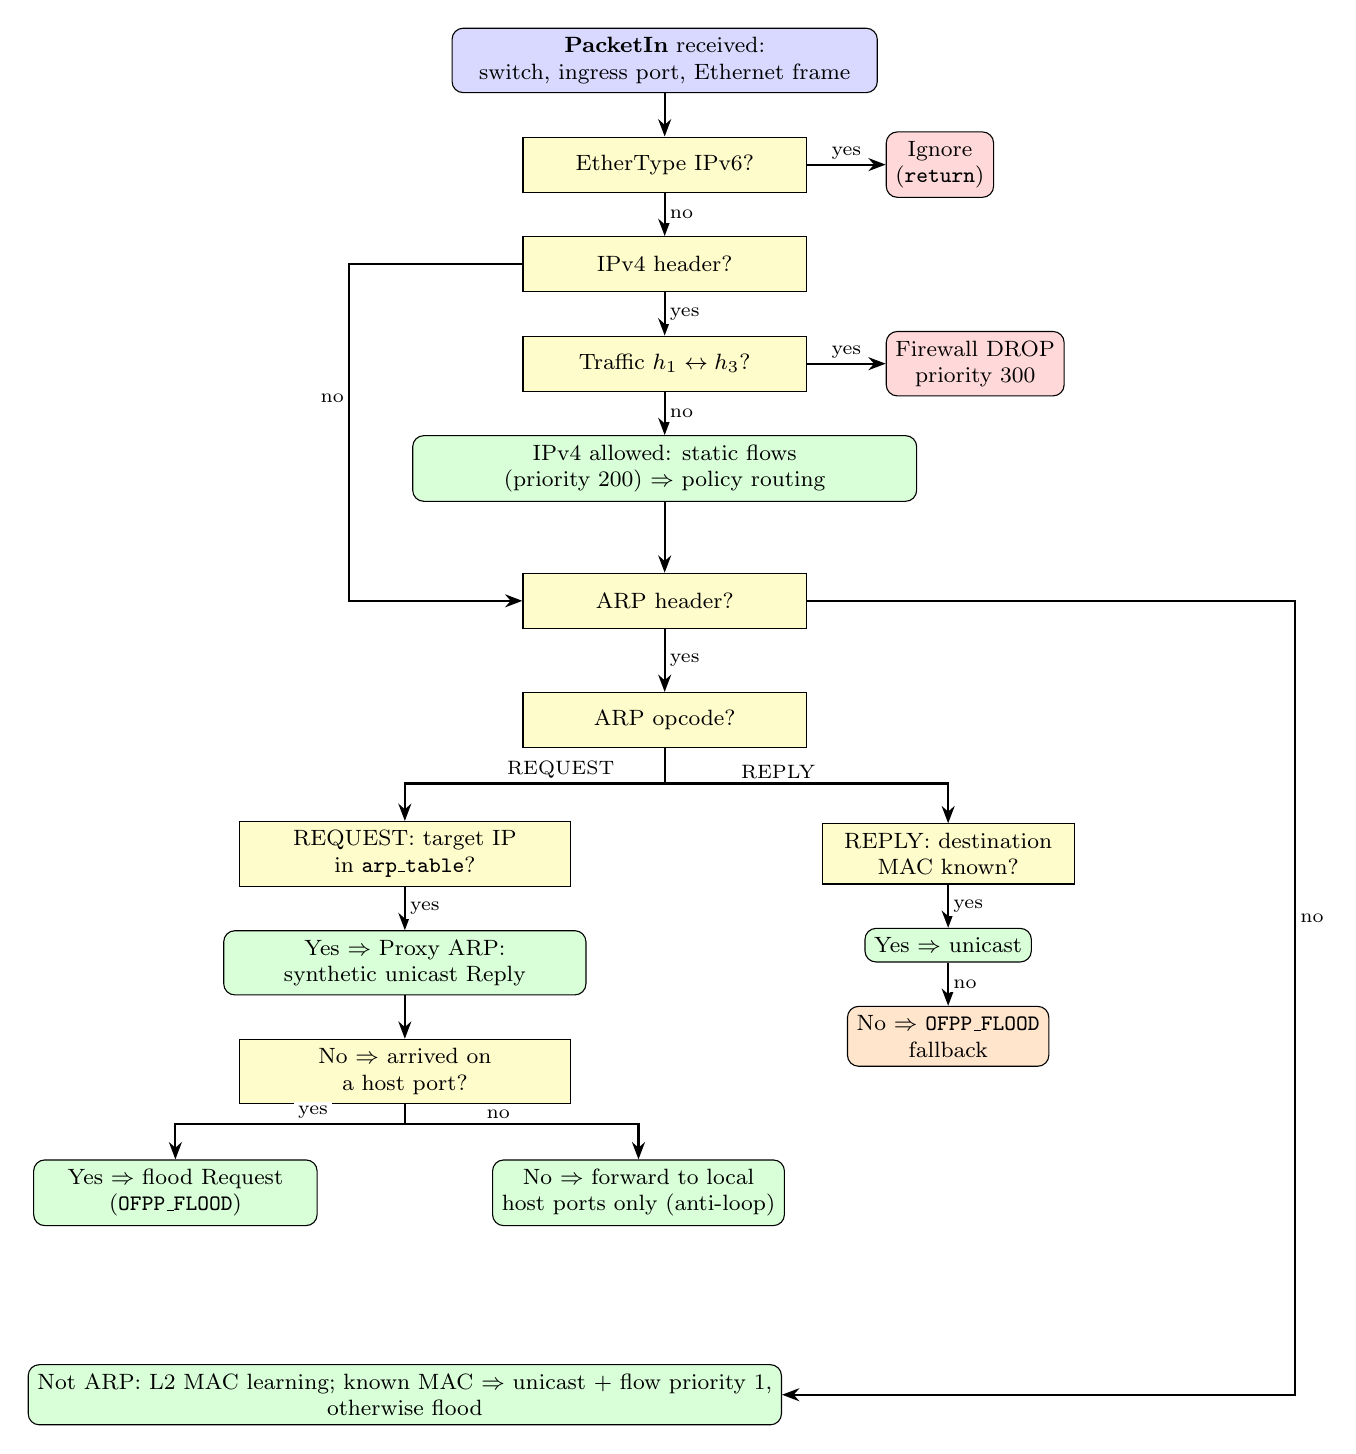
\begin{tikzpicture}[
  node distance=0.55cm and 1.0cm,
  start/.style={draw,rounded corners,fill=blue!15,align=center,font=\footnotesize,minimum width=5.4cm},
  dec/.style={draw,fill=yellow!20,align=center,font=\footnotesize,minimum width=3.6cm,minimum height=0.7cm},
  act/.style={draw,rounded corners,fill=green!15,align=center,font=\footnotesize},
  stop/.style={draw,rounded corners,fill=red!15,align=center,font=\footnotesize},
  fb/.style={draw,rounded corners,fill=orange!20,align=center,font=\footnotesize},
  ar/.style={-{Stealth[length=2.2mm]},thick},
  yn/.style={font=\scriptsize,inner sep=1.5pt,fill=white}
]
\node[start] (pi) {\textbf{PacketIn} received:\\switch, ingress port, Ethernet frame};
\node[dec,below=of pi] (v6) {EtherType IPv6?};
\node[stop,right=of v6] (drop6) {Ignore\\(\code{return})};
\node[dec,below=of v6] (ip) {IPv4 header?};
\node[dec,below=of ip] (fw) {Traffic $h_1\leftrightarrow h_3$?};
\node[stop,right=of fw] (fwd) {Firewall DROP\\priority 300};
\node[act,below=of fw,minimum width=6.4cm] (rt) {IPv4 allowed: static flows\\(priority 200) $\Rightarrow$ policy routing};
\node[dec,below=0.9cm of rt] (arp) {ARP header?};
\node[dec,below=0.8cm of arp] (op) {ARP opcode?};
\node[dec,minimum width=4.2cm] (req) at ($(op)+(-3.3,-1.7)$) {REQUEST: target IP\\in \code{arp\_table}?};
\node[dec,minimum width=3.2cm] (rep) at ($(op)+(3.6,-1.7)$) {REPLY: destination\\MAC known?};
\node[act,below=of req,minimum width=4.6cm] (px) {Yes $\Rightarrow$ Proxy ARP:\\synthetic unicast Reply};
\node[dec,below=of px,minimum width=4.2cm] (hp) {No $\Rightarrow$ arrived on\\a host port?};
\node[act,below left=0.7cm and -1.0cm of hp,minimum width=3.6cm] (fl) {Yes $\Rightarrow$ flood Request\\(\code{OFPP\_FLOOD})};
\node[act,below right=0.7cm and -1.0cm of hp,minimum width=3.6cm] (lo) {No $\Rightarrow$ forward to local\\host ports only (anti-loop)};
\node[act,below=of rep] (uni) {Yes $\Rightarrow$ unicast};
\node[fb,below=of uni] (ff) {No $\Rightarrow$ \code{OFPP\_FLOOD}\\fallback};
\node[act,below=3.3cm of hp,minimum width=8.4cm] (ml) {Not ARP: L2 MAC learning; known MAC $\Rightarrow$ unicast + flow priority 1,\\otherwise flood};

\draw[ar] (pi) -- (v6);
\draw[ar] (v6) -- node[yn,above]{yes} (drop6);
\draw[ar] (v6) -- node[yn,right]{no} (ip);
\draw[ar] (ip) -- node[yn,right]{yes} (fw);
\draw[ar] (fw) -- node[yn,above]{yes} (fwd);
\draw[ar] (fw) -- node[yn,right]{no} (rt);
\draw[ar] (rt) -- (arp);
\draw[ar] (ip.west) -- ++(-2.2,0) |- node[yn,pos=0.2,left]{no} (arp.west);
\draw[ar] (arp) -- node[yn,right]{yes} (op);
\draw[ar] (arp.east) -- ++(6.2,0) |- node[yn,pos=0.2,right]{no} (ml.east);
\draw[ar] (op.south) -- ++(0,-0.45) -| node[yn,pos=0.2,above]{REQUEST} (req.north);
\draw[ar] (op.south) -- ++(0,-0.45) -| node[yn,pos=0.2,above]{REPLY} (rep.north);
\draw[ar] (req) -- node[yn,right]{yes} (px);
\draw[ar] (px) -- (hp);
\draw[ar] (hp.south) -- ++(0,-0.25) -| node[yn,pos=0.2,above]{yes} (fl.north);
\draw[ar] (hp.south) -- ++(0,-0.25) -| node[yn,pos=0.2,above]{no} (lo.north);
\draw[ar] (rep) -- node[yn,right]{yes} (uni);
\draw[ar] (uni) -- node[yn,right]{no} (ff);
\end{tikzpicture}
\caption{Block diagram of the Ryu controller logic. It summarises the handling
of IPv6 packets, the firewall check between $h_1$ and $h_3$, IPv4 policy routing,
ARP Requests (controlled flooding and Proxy ARP), forwarding of ARP Replies and
the fallback MAC learning.}
\label{fig:flowchart}
\end{figure}

\subsection{Step 1: Identifying hosts and switches}
The first change is the definition of the constants that identify the endpoints
and the switches involved in the policy:

\begin{lstlisting}[style=py,caption={Constants for Task 3}]
IP_H1 = "10.0.0.10"
IP_H2 = "10.0.0.20"

DPID_S1 = 1
DPID_S2 = 2
DPID_S3 = 3
\end{lstlisting}

\code{IP\_H1} and \code{IP\_H2} identify the two hosts the policy applies to.
\code{DPID\_S1}, \code{DPID\_S2} and \code{DPID\_S3} identify the OpenFlow
switches. The DPID is received by the controller when a switch connects and
makes it possible to install every rule on the correct device.

\subsection{Step 2: The policy-routing map}
The dictionary \code{STATIC\_ROUTES} is the centralised representation of the
routing policy defined in the controller. Each key is a triple
\[
  (\text{switch DPID},\ \text{source IP},\ \text{destination IP})
\]
and the value is the OpenFlow output port to use on that switch.

\begin{lstlisting}[style=py,caption={Asymmetric static routing policy}]
STATIC_ROUTES = {
    # Forward: H1 -> S1 -> S3 -> S2 -> H2
    (DPID_S1, IP_H1, IP_H2): 4,
    (DPID_S3, IP_H1, IP_H2): 2,
    (DPID_S2, IP_H1, IP_H2): 2,

    # Return: H2 -> S2 -> S1 -> H1
    (DPID_S2, IP_H2, IP_H1): 1,
    (DPID_S1, IP_H2, IP_H1): 2,
}
\end{lstlisting}

The dictionary is consumed by \code{\_install\_static\_routes(datapath)}, which
is called from the \code{switch\_features\_handler} that Ryu runs when a switch
completes its OpenFlow connection. To change the path of a flow it is therefore
not necessary to change the controller's general logic: it is enough to modify
or add the corresponding entry in the dictionary, since the same installation
code reads every entry and turns it into the matching OpenFlow flow rule.

\subsection{Step 3: Proactive installation of the flow rules}
The routes are installed when a switch establishes its OpenFlow connection with
the controller. This lowers the latency of the first IP packet and guarantees
that the path is already available before communication starts.

\begin{lstlisting}[style=py,caption={Installing the table-miss rule and the static routes}]
@set_ev_cls(ofp_event.EventOFPSwitchFeatures, CONFIG_DISPATCHER)
def switch_features_handler(self, ev):
    datapath = ev.msg.datapath
    ofproto = datapath.ofproto
    parser = datapath.ofproto_parser

    match = parser.OFPMatch()
    actions = [parser.OFPActionOutput(ofproto.OFPP_CONTROLLER,
                                      ofproto.OFPCML_NO_BUFFER)]
    self._add_flow(datapath, priority=0, match=match, actions=actions)

    self._install_static_routes(datapath)
\end{lstlisting}

The decorator \code{@set\_ev\_cls(...EventOFPSwitchFeatures...)} makes the
function run during the OpenFlow connection set-up phase. The first rule,
priority~0, is the table-miss rule: any packet not matched by the other rules is
sent to the controller. \code{\_install\_static\_routes(datapath)} installs the
policy-routing rules on the switch that has just connected:

\begin{lstlisting}[style=py,caption={Proactive installation of the routes}]
def _install_static_routes(self, datapath):
    parser = datapath.ofproto_parser
    dpid = datapath.id

    for (sw_dpid, src_ip, dst_ip), out_port in STATIC_ROUTES.items():
        if sw_dpid != dpid:
            continue

        match = parser.OFPMatch(
            eth_type=0x0800,
            ipv4_src=src_ip,
            ipv4_dst=dst_ip
        )
        actions = [parser.OFPActionOutput(out_port)]
        self._add_flow(datapath, priority=200,
                       match=match, actions=actions)
\end{lstlisting}

\code{dpid = datapath.id} identifies the current switch. The loop walks all
entries of \code{STATIC\_ROUTES}; the test \code{if sw\_dpid != dpid} avoids
installing on one switch rules meant for another (when $s_1$ connects, the
entries of $s_2$ and $s_3$ are skipped); \code{continue} only skips the current
entry and moves on to the next one. For each relevant route an IPv4 match is
built with \code{eth\_type=0x0800}, \code{ipv4\_src} and \code{ipv4\_dst}, and
\code{OFPActionOutput(out\_port)} forwards the packet to the port defined by the
policy.

The routes have priority~200, which is lower than the priority~300 of the
Task~2 firewall, so a security policy always takes precedence over routing.
Priority~200 is, however, higher than the MAC-learning rules (priority~1) and
the table-miss rule (priority~0), so the path imposed in Task~3 prevails over
generic Ethernet forwarding.

\subsection{Step 4: Why ARP handling is needed}
The Task~3 routes match IPv4 packets only (\code{eth\_type=0x0800}). Before
sending an IP packet to $h_2$, however, $h_1$ must know its MAC address, and it
does so with an ARP request, which uses \code{eth\_type=0x0806}. The ARP request
therefore does not match the policy-routing rules: it hits the table-miss rule
and is sent to the controller, where the ARP logic handles it.

With the addition of $s_3$ the ring $s_1 - s_2 - s_3 - s_1$ exists. Standard
Ethernet flooding may make the same broadcast frame circulate repeatedly in the
ring, creating a Layer-2 loop or broadcast storm. For this reason a
controller-managed ARP handling was implemented.

\subsection{Example: ARP on the ring topology}
To understand the effect of the ring, consider $h_1$ pinging $h_2$.

\begin{figure}[H]
\centering
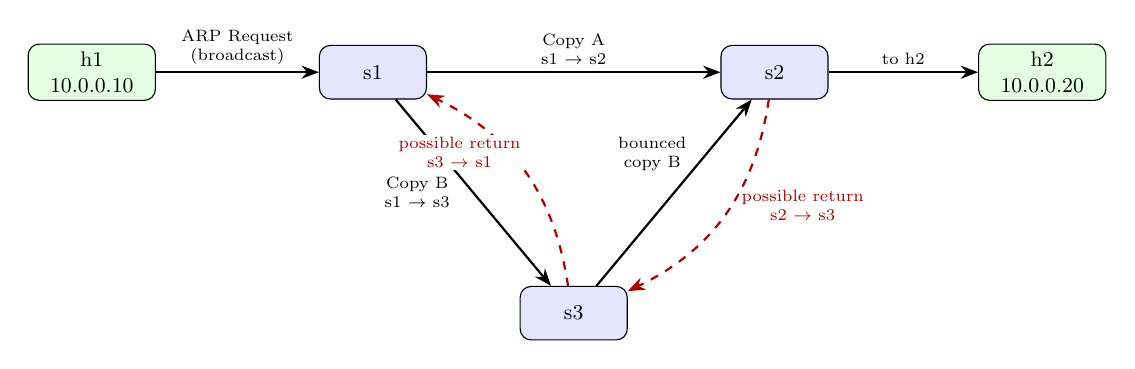
\begin{tikzpicture}[scale=0.85, every node/.style={transform shape},
  n/.style={draw,rounded corners,fill=blue!10,minimum width=1.6cm,minimum height=0.8cm,font=\small},
  h/.style={draw,rounded corners,fill=green!10,minimum width=1.9cm,minimum height=0.8cm,font=\small,align=center},
  ar/.style={-{Stealth[length=2.2mm]},thick},
  lp/.style={-{Stealth[length=2.2mm]},thick,red!70!black,dashed},
  lb/.style={font=\scriptsize,fill=white,inner sep=1pt,align=center}
]
\node[h] (h1) at (0,0) {h1\\10.0.0.10};
\node[n] (s1) at (4.2,0) {s1};
\node[n] (s2) at (10.2,0) {s2};
\node[h] (h2) at (14.2,0) {h2\\10.0.0.20};
\node[n] (s3) at (7.2,-3.6) {s3};

\draw[ar] (h1) -- node[lb,above=2pt]{ARP Request\\(broadcast)} (s1);
\draw[ar] (s1) -- node[lb,above=2pt]{Copy A\\s1 $\to$ s2} (s2);
\draw[ar] (s2) -- node[lb,above=2pt]{to h2} (h2);
\draw[ar] (s1) -- node[lb,below left=0pt and 2pt,pos=0.4]{Copy B\\s1 $\to$ s3} (s3);
\draw[ar] (s3) -- node[lb,above left=0pt and 0pt,pos=0.6]{bounced\\copy B} (s2);
\draw[lp] (s3) to[bend right=28] node[lb,above left,pos=0.5,text=red!70!black]{possible return\\s3 $\to$ s1} (s1);
\draw[lp] (s2) to[bend left=28] node[lb,right=3pt,pos=0.45,text=red!70!black]{possible return\\s2 $\to$ s3} (s3);
\end{tikzpicture}
\caption{ARP flooding on the ring. The broadcast sent by $h_1$ can be duplicated
by $s_1$ and propagated towards both $s_2$ and $s_3$. Dashed red arrows show the
possible circulation of the broadcast around the ring when it is not
controlled.}
\label{fig:arp-ring}
\end{figure}

\begin{enumerate}
  \item $h_1$ sends a broadcast ARP Request to $s_1$. The frame has Ethernet
        destination \code{ff:ff:ff:ff:ff:ff}, so $s_1$ cannot forward it to a
        single known port.
  \item $s_1$ generates a \code{PACKET\_IN} towards Ryu containing the ARP
        Request.
  \item Ryu records the association $h_1\to s_1$, port~2 in its
        \code{mac\_to\_port} table.
  \item Since $s_1$ has two links to the other switches of the ring, an
        uncontrolled \code{FLOOD} \code{PACKET\_OUT} produces two copies of the
        same request:
        \begin{itemize}
          \item Copy A: sent by $s_1$ to $s_2$;
          \item Copy B: sent by $s_1$ to $s_3$.
        \end{itemize}
  \item Copy A reaches $s_2$ from the port connected to $s_1$. If $s_2$ kept
        flooding on all its ports (including the one towards $s_3$), the
        request would continue around the ring instead of stopping once it has
        reached $h_2$.
  \item Likewise, Copy B reaches $s_3$ from the port connected to $s_1$. If
        $s_3$ flooded on all ports it would send another copy to $s_2$.
  \item At this point $s_2$ may receive the same ARP Request for $h_1$ twice:
        once through $s_1$ (Copy A) and once through $s_3$ (the bounced Copy B).
        Each time the Ethernet source field of the frame is the same: the MAC of
        $h_1$.
  \item Every copy received by a new switch generates a new \code{PACKET\_IN}
        towards Ryu. Executing the same learning statement used for legitimate
        traffic,
        \begin{lstlisting}[style=py]
self.mac_to_port[dpid][src_mac] = in_port
        \end{lstlisting}
        the controller updates its table every time it receives a new
        \code{PACKET\_IN}, even if it is a duplicate copy of the original
        broadcast.
  \item Because an Ethernet frame has no TTL field like an IP packet, the same
        request keeps circulating in the ring, re-entering the same switches
        from different ports.
\end{enumerate}

The \code{mac\_to\_port} table of Ryu associates each MAC with a single port per
switch, i.e.\ it only records the \emph{last} port from which that MAC was
observed:
\[
  \code{mac\_to\_port[dpid][MAC h1]} = \text{last observed port}
\]
Suppose $s_3$ sees the MAC of $h_1$ for the first time arriving from the port
connected to $s_1$ (Copy B, direct path). Ryu records
\code{mac\_to\_port[s3][MAC h1]} $=$ port towards $s_1$. If, because of the
re-entry in the ring, the same MAC later also arrives at $s_3$ from the port
connected to $s_2$ (because Copy A went around $s_1\to s_2\to s_3$), Ryu
overwrites the previous association with the port towards $s_2$. At this point
the controller's state is corrupted: Ryu believes $h_1$ is behind the port
connecting $s_3$ to $s_2$, although $h_1$ was never moved.

This phenomenon is known as \emph{MAC flapping}: the same MAC address seems to
``jump'' from one port to another, because the controller observes copies of the
same broadcast frame arriving from different directions of the ring and cannot
tell which port represents the real position of the host. The practical
consequences are similar to those of a broadcast storm in a legacy Ethernet
network without STP:
\begin{itemize}
  \item future replies destined to $h_1$ may be forwarded on the wrong port, i.e.\
        towards the other switch of the ring instead of the host;
  \item the number of \code{PACKET\_IN} messages processed by the controller
        grows needlessly, increasing the load on Ryu;
  \item the table does not converge to a stable state but is rewritten at every
        new lap of the broadcast;
  \item in the extreme case, the same ARP request may circulate indefinitely
        among $s_1$, $s_2$ and $s_3$, saturating the links.
\end{itemize}

\subsection{Step 5: Defining the inter-switch ports}
In the proposed solution, Ryu controls the propagation of ARP requests by
distinguishing the ports that connect to switches from those that connect to
hosts. This information is stored in the dictionary \code{SWITCH\_PORTS}:

\begin{lstlisting}[style=py,caption={Inter-switch ports used to control ARP flooding}]
SWITCH_PORTS = {
    DPID_S1: {3, 4},   # 3 = s2, 4 = s3
    DPID_S2: {1, 4},   # 1 = s1, 4 = s3
    DPID_S3: {1, 2},   # 1 = s1, 2 = s2
}
\end{lstlisting}

\subsection{Step 6: ARP handling logic}
\subsubsection{Controlled flooding of ARP Requests}
When an ARP Request enters from a host port, the controller propagates it into
the network so that the target can receive it. When the request instead arrives
from an inter-switch port, the controller does not send it to the other
switches: it forwards it only to the local host ports. In this way the request
can reach $h_2$ but cannot keep bouncing along the ring. Flooding is thus
limited to the first traversal of the network and does not turn into a circular
Layer-2 propagation.

\subsubsection{Learning IP--MAC associations}
While processing ARP messages, the controller stores IP--MAC associations in
\code{arp\_table}, e.g.\ \code{10.0.0.20} $\to$ MAC of $h_2$. During the first
communication attempt between $h_1$ and $h_2$ this association is not yet
available. The ARP Request of $h_1$ must therefore be propagated with controlled
flooding until it reaches $h_2$, which generates the normal unicast ARP Reply
towards $h_1$; the controller learns the IP--MAC association by observing that
message. After this exchange both $h_1$ and the controller know the MAC of
$h_2$.

\subsubsection{ARP Reply handling and Proxy ARP}
After the first ARP resolution the association between the IP of $h_2$ and its
MAC is stored both in the ARP cache of $h_1$ and in the controller's
\code{arp\_table}. Subsequent ICMP packets therefore need no new ARP Request:
$h_1$ can use the MAC it already learned. Proxy ARP comes into play only if
$h_1$ generates a new ARP request, for instance after its ARP cache entry
expires or is deleted. If the requested IP is already in \code{arp\_table}, Ryu
uses the MAC learned earlier to build a synthetic ARP Reply and sends it
directly, unicast, to $h_1$. The controller thus avoids propagating the
broadcast on the ring again.

Controlled flooding is therefore used when the IP--MAC association is not yet
known, whereas Proxy ARP is used for later requests, when the controller already
has the needed information.

\subsection{Step 7: Implementing the ARP logic}
\subsubsection{ARP table and IP--MAC learning}
A global ARP table that stores IP $\to$ MAC associations was added to the
controller's constructor:

\begin{lstlisting}[style=py,caption={Global ARP table of the controller}]
self.arp_table = {}
\end{lstlisting}

\begin{lstlisting}[style=py,caption={Learning ARP information}]
arp_pkt = pkt.get_protocol(arp.arp)
if arp_pkt:
    src_mac = arp_pkt.src_mac
    src_ip = arp_pkt.src_ip
    dst_ip = arp_pkt.dst_ip

    self.arp_table[src_ip] = src_mac
    self.mac_to_port[dpid][src_mac] = in_port
\end{lstlisting}

When the controller receives an ARP packet it extracts the needed addresses and
updates both the ARP table and the MAC-learning table.

\subsubsection{Proxy ARP}
If the requested IP address is already in \code{arp\_table}, the controller does
not have to propagate the broadcast request on the ring again. Ryu uses the MAC
already learned to build a synthetic ARP Reply and sends it directly to the
requesting host in a \code{PacketOut} message.

\begin{lstlisting}[style=py,caption={Proxy ARP when the MAC is known}]
if dst_ip in self.arp_table:
    reply_mac = self.arp_table[dst_ip]
    e = ethernet.ethernet(dst=src_mac, src=reply_mac,
                          ethertype=0x0806)
    a = arp.arp(opcode=arp.ARP_REPLY,
                src_mac=reply_mac, src_ip=dst_ip,
                dst_mac=src_mac, dst_ip=src_ip)
    p = packet.Packet()
    p.add_protocol(e)
    p.add_protocol(a)
    p.serialize()
    self._packet_out(datapath, ofproto.OFPP_CONTROLLER,
                     [parser.OFPActionOutput(in_port)], p.data)
    return
\end{lstlisting}

Proxy ARP is used only when a new ARP request is generated for an IP already
known to the controller. The following IPv4 packets of the communication do not
need a new ARP request, because the host already holds the destination MAC in
its cache.

\subsubsection{Controlled flooding of ARP Requests}
If the requested IP is not yet in \code{arp\_table}, the controller must let the
request reach the destination host. How it is forwarded depends on the port the
request entered the switch from.

\begin{lstlisting}[style=py,caption={Controlled ARP flooding}]
sw_ports = SWITCH_PORTS.get(dpid, set())

if in_port not in sw_ports:
    actions = [parser.OFPActionOutput(ofproto.OFPP_FLOOD)]
    self._packet_out(datapath, in_port, actions, msg.data,
                     msg.buffer_id)
else:
    host_ports = [p_num for p_num in range(1, 5)
                  if p_num not in sw_ports]
    for hp in host_ports:
        if hp != in_port:
            self._packet_out(datapath, in_port,
                             [parser.OFPActionOutput(hp)],
                             msg.data)
return
\end{lstlisting}

If the ARP request enters from a host port, the controller floods it into the
network so that it can reach hosts attached to other switches. If instead it
enters from an inter-switch port, it has already crossed at least one link of
the network; the controller then sends it only to the local host ports and does
not forward it to other switches. This breaks the possible circulation of the
broadcast along the ring.

\subsubsection{Forwarding ARP Replies}
When $h_2$ receives the ARP Request it generates a unicast ARP Reply towards
$h_1$. The reply reaches the Ryu controller through a new \code{PacketIn}. The
controller updates \code{mac\_to\_port} with the port where it saw the source MAC
and checks whether it knows the port associated with the MAC of $h_1$. If so,
Ryu forwards the unicast ARP Reply to the corresponding port. If the destination
MAC is not yet known, the code falls back on \code{OFPP\_FLOOD}. On a ring this
case needs care, because flooding the ARP Reply does not apply the inter-switch
port filter and may generate copies of the frame on the ring.

\begin{lstlisting}[style=py,caption={Forwarding an ARP reply}]
elif arp_pkt.opcode == arp.ARP_REPLY:
    self.mac_to_port[dpid][src] = in_port
    if dst in self.mac_to_port[dpid]:
        out_port = self.mac_to_port[dpid][dst]
        self._packet_out(datapath, in_port,
                         [parser.OFPActionOutput(out_port)],
                         msg.data, msg.buffer_id)
    else:
        self._packet_out(datapath, in_port,
                         [parser.OFPActionOutput(ofproto.OFPP_FLOOD)],
                         msg.data, msg.buffer_id)
    return
\end{lstlisting}

\subsection{Step 8: Generic MAC learning}
Generic MAC learning is the controller's fallback behaviour for Ethernet frames
not handled by the previous policies.

\begin{lstlisting}[style=py,caption={Generic MAC learning}]
self.mac_to_port[dpid][src] = in_port
out_port = (self.mac_to_port[dpid][dst]
            if dst in self.mac_to_port[dpid]
            else ofproto.OFPP_FLOOD)
actions = [parser.OFPActionOutput(out_port)]

if out_port != ofproto.OFPP_FLOOD:
    match = parser.OFPMatch(in_port=in_port,
                            eth_dst=dst,
                            eth_src=src)
    self._add_flow(datapath, priority=1,
                   match=match, actions=actions)
\end{lstlisting}

When it receives an Ethernet frame, the controller associates the source MAC
with the ingress port of the current switch. If the destination MAC is already
in the table, the frame is forwarded unicast on the corresponding port;
otherwise flooding is used as the fallback. When the output port is known, the
controller also installs a flow rule with priority~1, so that later frames with
the same MAC pair are forwarded directly by the switch without generating more
\code{PacketIn} messages.

Priority~1 is lower than both the priority-300 firewall rules and the
priority-200 policy-routing rules. MAC learning therefore cannot alter the path
imposed by the more specific policies; it only acts as a general mechanism for
traffic not covered by them.

\begin{table}[H]
\centering
\begin{tabular}{clp{7cm}}
\toprule
Priority & Rule & Installed\\
\midrule
300 & Firewall $h_1\leftrightarrow h_3$ (drop) & reactively, on first offending packet\\
200 & Static policy routing & proactively, at switch connection\\
1 & MAC learning & reactively, when destination known\\
0 & Table-miss (to controller) & proactively, at switch connection\\
\bottomrule
\end{tabular}
\caption{Flow-rule priorities used by the controller}
\end{table}

%====================================================================
\section{Experimental Validation and Results}
%====================================================================
\subsection{Test environment and methodology}
The tests were run in the Kathar\'a topology made of the OpenFlow switches
$s_1$, $s_2$ and $s_3$, the Ryu controller, the hosts $h_1$, $h_2$, $h_3$ and
\code{ext1}, and the router $r_1$. The tests verify the selective block between
$h_1$ and $h_3$, the reachability of $h_2$, the asymmetric path imposed on IPv4
traffic, and the correct behaviour of the ARP handling on the ring.

Before each test the topology was started and the switches were connected to the
controller. Command outputs were collected on the nodes involved and compared
with the Open vSwitch flow tables.

\textbf{Note on the screenshots.} The terminal captures in this section were
taken with an earlier revision of the controller whose log messages were in
Italian: \emph{``porta''} means \emph{port} and \emph{``Switch connesso''} means
\emph{switch connected}. The controller logic is identical; only the wording of
the log strings was translated to English in the final source code.

\subsection{Controller start-up and switch connection}
As a first check, the Ryu controller was started on OpenFlow TCP port 6653. The
purpose is to confirm that the application loads correctly, that the three
OpenFlow switches connect, and that the IPv4 routes defined in
\code{STATIC\_ROUTES} are installed proactively.

\begin{figure}[H]
\centering
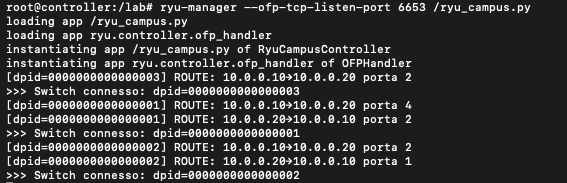
\includegraphics[width=0.85\linewidth]{screenshots/controller_startup.png}
\caption{Ryu controller output at start-up. The messages confirm the connection
of $s_1$, $s_2$ and $s_3$ and the proactive installation of the static
policy-routing routes.}
\end{figure}

The output confirms that the three switches are recognised: $s_1$ has DPID~1,
$s_2$ has DPID~2 and the new switch $s_3$ has DPID~3. For each device the
\code{ROUTE} message is printed while \code{\_install\_static\_routes()} runs, so
the policy-routing flow rules are installed at OpenFlow connection time, before
any IP packet is generated. In particular, $h_1\to h_2$ traffic is configured
towards port~4 on $s_1$, port~2 on $s_3$ and port~2 on $s_2$, while the return
traffic $h_2\to h_1$ is configured towards port~1 on $s_2$ and port~2 on $s_1$.
The absence of a return route on $s_3$ confirms the expected asymmetric
behaviour.

\subsection{Initial state of the flow tables}
Right after the switches connect to the controller, and before generating any
test traffic, the flow tables of $s_1$, $s_2$ and $s_3$ were inspected with:
\begin{lstlisting}[style=sh]
ovs-ofctl -O OpenFlow13 dump-flows sX
\end{lstlisting}

\begin{figure}[H]
\centering
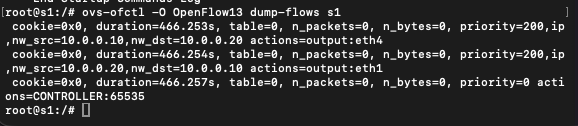
\includegraphics[width=\linewidth]{screenshots/flows_s1_initial.png}
\caption{Flow table of $s_1$ right after connecting to the controller, before
any test traffic.}
\end{figure}
\begin{figure}[H]
\centering
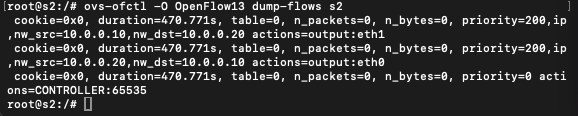
\includegraphics[width=\linewidth]{screenshots/flows_s2_initial.png}
\caption{Flow table of $s_2$ right after connecting to the controller, before
any test traffic.}
\end{figure}
\begin{figure}[H]
\centering
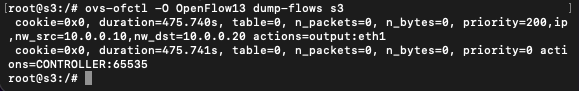
\includegraphics[width=\linewidth]{screenshots/flows_s3_initial.png}
\caption{Flow table of $s_3$ right after connecting to the controller, before
any test traffic.}
\end{figure}

The output confirms that the policy-routing flows are already present at
OpenFlow connection time, without any IP packet having been sent by the hosts.
Each switch contains only two kinds of rules: the priority-200 policy-routing
flow and the priority-0 table-miss rule. All counters read
\code{n\_packets=0} and \code{n\_bytes=0}, meaning that none of the rules has
yet received matching traffic: the mere presence of the flows demonstrates the
proactive installation, independent of the traffic generated by the hosts.

\subsection{Connectivity tests and firewall verification}
After checking the initial installation of the static routes, the following
connectivity tests were run. They verify that traffic between $h_1$ and $h_2$ is
allowed, that communication between $h_1$ and $h_3$ is blocked in both
directions, and that $h_2$ remains reachable.

\begin{lstlisting}[style=sh,caption={Commands used for the connectivity and firewall tests}]
# h1 terminal: connectivity allowed towards h2
ping -c 4 10.0.0.20

# h1 terminal: forbidden traffic towards h3
ping -c 4 -W 1 10.0.0.30

# h3 terminal: check the block in the opposite direction
ping -c 4 -W 1 10.0.0.10

# h2 terminal: h2 must stay reachable from both hosts
ping -c 4 10.0.0.10
ping -c 4 10.0.0.30

# switch terminals: check the flows after the tests
ovs-ofctl -O OpenFlow13 dump-flows s1
ovs-ofctl -O OpenFlow13 dump-flows s2
ovs-ofctl -O OpenFlow13 dump-flows s3
\end{lstlisting}

\begin{figure}[H]
\centering
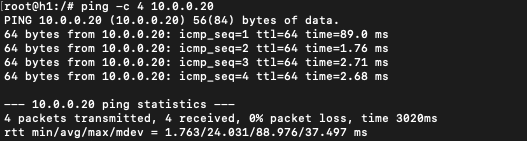
\includegraphics[width=0.8\linewidth]{screenshots/ping_h1_h2.png}
\caption{Allowed connectivity: $h_1$ reaches $h_2$.}
\end{figure}
\begin{figure}[H]
\centering
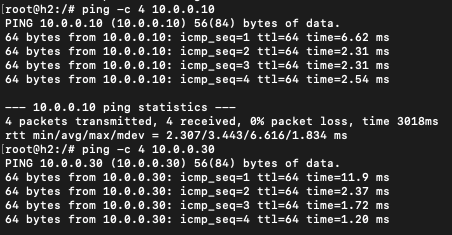
\includegraphics[width=0.75\linewidth]{screenshots/ping_h2_h1_h3.png}
\caption{Allowed connectivity: $h_2$ communicates correctly with $h_1$ and
$h_3$.}
\end{figure}
\begin{figure}[H]
\centering
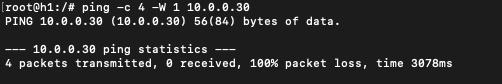
\includegraphics[width=0.75\linewidth]{screenshots/ping_h1_h3_blocked.png}\\[0.4em]
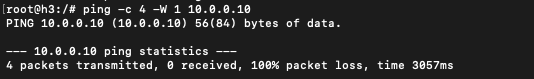
\includegraphics[width=0.75\linewidth]{screenshots/ping_h3_h1_blocked.png}\\[0.4em]
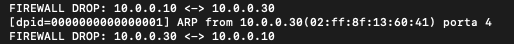
\includegraphics[width=0.75\linewidth]{screenshots/firewall_drop_log.png}
\caption{Bidirectional firewall test: ICMP traffic between $h_1$ and $h_3$ is
blocked in both directions (100\% packet loss), and the controller logs the
\code{FIREWALL DROP} events.}
\end{figure}
\begin{figure}[H]
\centering
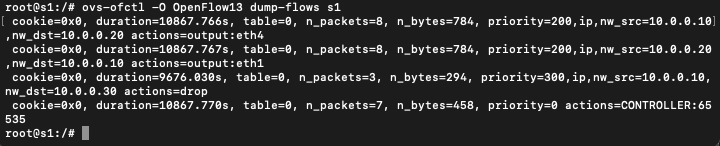
\includegraphics[width=\linewidth]{screenshots/flows_s1_after_tests.png}\\[0.4em]
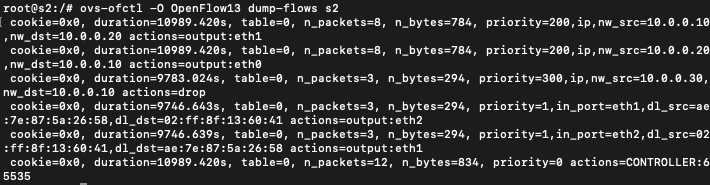
\includegraphics[width=\linewidth]{screenshots/flows_s2_after_tests.png}\\[0.4em]
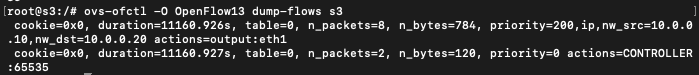
\includegraphics[width=\linewidth]{screenshots/flows_s3_after_tests.png}
\caption{Reactive firewall flow rules (priority 300, action drop) installed after
the communication attempts between $h_1$ and $h_3$, shown for $s_1$, $s_2$ and
$s_3$. On the path considered the drop already happens at $s_1$, so $s_3$ shows
no flow specific to $h_1\leftrightarrow h_3$.}
\end{figure}

The results confirm that the firewall policy is selective and bidirectional:
communication between $h_1$ and $h_3$ is blocked, while $h_2$ remains reachable
by the other hosts. The flow tables also show that, after the first forbidden
communication attempt, the controller installs flow rules with priority~300 and
action drop. These rules take precedence over the static policy-routing routes,
which have priority~200.

\subsubsection{Proxy ARP verification}
During a new communication attempt from $h_1$ to $h_3$ the controller receives an
ARP request coming from $h_1$, as shown by the following messages:

\begin{lstlisting}[caption={Controller messages for the ARP request}]
[dpid=0000000000000001] ARP from 10.0.0.10(a2:f1:4a:2d:12:c5) port 2
[dpid=0000000000000001] ARP PROXY REPLY: 10.0.0.30 is f2:07:e4:cc:a5:7b
\end{lstlisting}

The first line says that switch $s_1$, with DPID~1, received on OpenFlow port~2 an
ARP request generated by $h_1$. The request concerns the IP address of $h_3$,
10.0.0.30. The controller already has in \code{arp\_table} the association
between 10.0.0.30 and MAC \code{f2:07:e4:cc:a5:7b}. Consequently, instead of
forwarding the ARP request as a broadcast over the ring, Ryu directly generates
a synthetic ARP Reply and sends it unicast to $h_1$. This is the Proxy ARP
mechanism.

A new ARP request can be generated even if the MAC of $h_3$ is already in the
cache of $h_1$, because the entry is in the \code{STALE} state. In this state the
Linux kernel keeps the IP--MAC association but may ask for a reachability check
of the neighbour. Proxy ARP supplies the association again without flooding the
inter-switch links.

\begin{figure}[H]
\centering
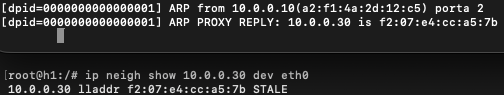
\includegraphics[width=0.9\linewidth]{screenshots/proxy_arp.png}
\caption{Proxy ARP verification. The terminal of $h_1$ shows the entry for $h_3$
in the STALE state; the controller log shows the ARP request being received and
the synthetic ARP Reply for 10.0.0.30 being generated.}
\end{figure}

\subsection{Verification of the asymmetric policy routing}
The asymmetric policy routing can be verified by analysing the switch flow
tables shown above. It is enough to identify the priority-200 IPv4 rules and read
the fields \code{nw\_src}, \code{nw\_dst} and the output action.

For the forward direction, the rules with \code{nw\_src=10.0.0.10} and
\code{nw\_dst=10.0.0.20} show that packets coming from $h_1$ are forwarded by
$s_1$ towards $s_3$, by $s_3$ towards $s_2$, and finally by $s_2$ towards $h_2$.
The resulting path is
\[
  h_1 \to s_1 \to s_3 \to s_2 \to h_2 .
\]
Conversely, for the return traffic, the rules with \code{nw\_src=10.0.0.20} and
\code{nw\_dst=10.0.0.10} show that packets are forwarded by $s_2$ directly to
$s_1$ and then to $h_1$. The reverse path is therefore
\[
  h_2 \to s_2 \to s_1 \to h_1 .
\]
The absence on $s_3$ of a flow with source 10.0.0.20 and destination 10.0.0.10
confirms that the return traffic does not cross that switch.

\subsection{TCP service tests: curl, iperf3 and tcpdump}
\subsubsection{curl: HTTP application check}
The \code{curl} command correctly returns the HTML page of web server $h_2$,
confirming that the HTTP service on port 8080 is reachable from the external
client \code{ext1}.

\subsubsection{iperf3: TCP connection and throughput}
The \code{iperf3} command also establishes a TCP connection with the server on
port 5201 and transfers data at an average rate of about 48.3~Mbit/s over the
measured interval. The test was interrupted manually after about seven seconds,
as the message \code{iperf3: interrupt} shows. The results therefore demonstrate
correct connectivity of the TCP services between the external network and the
internal web server.

\begin{figure}[H]
\centering
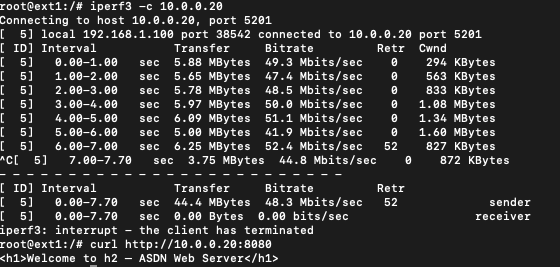
\includegraphics[width=0.8\linewidth]{screenshots/iperf_curl_ext1.png}
\caption{TCP service tests from \code{ext1}: data transfer with \code{iperf3} and
HTTP access to web server $h_2$ with \code{curl}.}
\end{figure}

\subsubsection{Capturing ARP traffic with tcpdump}
To observe directly the packets received by web server $h_2$, a capture was
started on its data interface \code{eth0}:
\begin{lstlisting}[style=sh,caption={Starting tcpdump on the data interface of $h_2$}]
tcpdump -i eth0
\end{lstlisting}
\code{tcpdump} intercepts and shows in real time the frames reaching the selected
interface. Here, \code{eth0} of $h_2$ is the interface attached to the data
domain with switch $s_2$, so the capture confirms the actual arrival of traffic
coming from the rest of the SDN network. While the capture was running, the
following command was executed on $h_1$:
\begin{lstlisting}[style=sh,caption={Ping to an unassigned IP address}]
ping -c 4 10.0.0.99
\end{lstlisting}
The address 10.0.0.99 is not assigned to any host of the topology. Before it can
send ICMP packets, $h_1$ must find the corresponding MAC address with ARP, so
broadcast requests of the following kind are generated:
\begin{lstlisting}[caption={ARP request generated by $h_1$}]
ARP, Request who-has 10.0.0.99 tell 10.0.0.10, length 46
\end{lstlisting}
As the figure shows, these ARP requests were observed in the capture on $h_2$.
The result confirms that $h_2$ receives the ARP broadcast frames generated by
$h_1$ and forwarded through the SDN network. Since no node has IP address
10.0.0.99, $h_2$ sends no ARP Reply; the \code{ping} on $h_1$ therefore ends with
\code{Destination Host Unreachable} messages and total packet loss. The purpose
of the test is to show that the ARP requests arrive at $h_2$, not that the
non-existent address is reachable.

\begin{figure}[H]
\centering
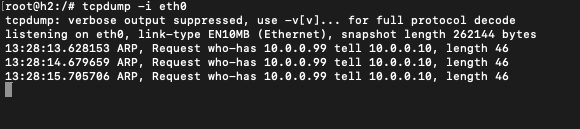
\includegraphics[width=0.85\linewidth]{screenshots/tcpdump_h2.png}
\caption{\code{tcpdump} capture on \code{eth0} of $h_2$. The ARP requests
\code{who-has 10.0.0.99 tell 10.0.0.10} show that the broadcast frames generated
by $h_1$ reach $h_2$.}
\end{figure}

\subsection{ARP and Proxy ARP handling}
\begin{figure}[H]
\centering
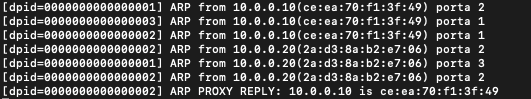
\includegraphics[width=0.7\linewidth]{screenshots/arp_log_first_ping.png}
\caption{Ryu controller log during the first ping from $h_1$ to $h_2$ after
restarting the topology.}
\end{figure}

After the containers are restarted, both the ARP caches of the hosts and the ARP
table of the Ryu controller are initially empty. When $h_1$ runs the first ping
to $h_2$ it cannot yet send the IPv4 packet directly: it first needs the MAC
address associated with 10.0.0.20, so it generates a broadcast ARP request.

The log lines in the Ryu console describe the ARP frames reaching the controller
through OpenFlow \code{PacketIn} messages. A line of the form
\begin{lstlisting}
[dpid=...] ARP from IP (MAC) port N
\end{lstlisting}
does \emph{not} represent a reply sent by the controller. It indicates that a
switch received an ARP frame on its OpenFlow port $N$ and sent it to Ryu for
processing. The \code{dpid} field identifies the switch that generated the
\code{PacketIn}; the IP field identifies the sender of the observed ARP request
or reply; the MAC in parentheses is the source MAC of the received frame. For
example, the message
\begin{lstlisting}
[dpid=0000000000000001] ARP from 10.0.0.10(ce:ea:70:f1:3f:49) port 2
\end{lstlisting}
indicates that switch $s_1$, DPID~1, received an ARP frame on port~2. The sender
is $h_1$, with IP 10.0.0.10 and MAC \code{ce:ea:70:f1:3f:49}. After the
\code{PacketIn}, the controller learns and stores the association
\code{10.0.0.10 -> ce:ea:70:f1:3f:49}. Similarly, the line
\begin{lstlisting}
[dpid=0000000000000001] ARP from 10.0.0.20(2a:d3:8a:b2:e7:06) port 3
\end{lstlisting}
shows that Ryu observed an ARP frame sent by $h_2$, so the controller also learns
\code{10.0.0.20 -> 2a:d3:8a:b2:e7:06}. The fact that the frame of $h_2$ is seen on
$s_1$ at port~3 does not mean that $h_2$ is physically attached to $s_1$: it
means that the ARP frame from $h_2$ crossed $s_2$ and reached $s_1$ over the
inter-switch link associated with port~3.

The final line has a different meaning:
\begin{lstlisting}
[dpid=0000000000000002] ARP PROXY REPLY: 10.0.0.10 is ce:ea:70:f1:3f:49
\end{lstlisting}
This line does not describe a received frame but a reply \emph{generated by the
controller}. Ryu received, through $s_2$, an ARP request asking for the MAC
associated with IP 10.0.0.10. Since the association
\code{10.0.0.10 -> ce:ea:70:f1:3f:49} had already been learned, the controller
does not forward the request as a broadcast again; it directly builds a synthetic
ARP Reply containing the requested information and sends it to $s_2$ in an
OpenFlow \code{PacketOut} message, and the switch finally forwards it unicast to
the host that made the request. The distinction between the two kinds of log line
is therefore:
\begin{itemize}
  \item \textbf{ARP from:} ARP frame received by the controller via
        \code{PacketIn}; Ryu learns the sender's IP--MAC association.
  \item \textbf{ARP PROXY REPLY:} ARP frame built by the controller and sent via
        \code{PacketOut}; Ryu supplies an IP--MAC association already present in
        its ARP table.
\end{itemize}

The advantage of Proxy ARP is not to make the ARP reply unicast, since an
ordinary ARP Reply generated by the target host is normally unicast as well.
The mechanism instead avoids propagating the broadcast ARP Request all the way to
the requested host and waiting for its reply. When the MAC is already known to
the controller, Ryu immediately generates a synthetic ARP Reply for the
requester, reducing resolution latency and broadcast traffic on the SDN ring.

%====================================================================
\section{Conclusions}
%====================================================================
The three tasks were implemented and verified on the Kathar\'a topology:
\begin{itemize}
  \item \textbf{Ring topology:} $s_3$ closes the loop $s_1 - s_2 - s_3 - s_1$.
        The loop is harmless because the controller never floods ARP blindly
        between switches.
  \item \textbf{Firewall:} IPv4 traffic between $h_1$ and $h_3$ is dropped in
        both directions by priority-300 flows, while $h_2$ remains reachable.
  \item \textbf{Policy routing:} $h_1\to h_2$ takes $s_1\to s_3\to s_2$ and
        $h_2\to h_1$ takes $s_2\to s_1$, using priority-200 flows installed
        proactively.
\end{itemize}

Known limitations of the current implementation: port numbers in
\code{STATIC\_ROUTES} and \code{SWITCH\_PORTS} are hard-coded for this topology;
firewall drop flows have no timeout; an ARP Reply with an unknown destination MAC
falls back to an unfiltered flood; and IPv6 is ignored. Natural extensions
would be topology discovery (e.g.\ Ryu's \code{--observe-links}) to compute
paths automatically, or failover to the direct $s_1$--$s_2$ link when the detour
through $s_3$ fails.

\end{document}
